\documentclass[aps,prmaterials,reprint,superscriptaddress,nofootinbib]{revtex4-2}

\usepackage[utf8]{inputenc}
\usepackage[T1]{fontenc}
\usepackage{graphicx}
\usepackage{amsmath,amssymb}
\usepackage{booktabs}
\usepackage{xcolor}
\usepackage[colorlinks=true,linkcolor=blue!50!black,citecolor=blue!50!black,urlcolor=blue!50!black]{hyperref}

\newcommand{\ddF}{\Delta\Delta F_{\mathrm{iso}}}
\newcommand{\ddG}{\Delta\Delta G_{\mathrm{iso}}}
\newcommand{\mA}{m\AA}
\newcommand{\OH}{O-H}
\newcommand{\OO}{O$\cdots$O}

\begin{document}

\title{A short-bond rule for the isotope effect on polymorph stability in hydrogen-bonded crystals}

\author{Muhammet Can Ergani\c{s}}
\homepage{https://orcid.org/0009-0001-1397-6366}
\affiliation{Department of Metallurgical and Materials Engineering, Middle East Technical University, Ankara, T\"urkiye}

\date{Draft of 23 October 2026}

\begin{abstract}
Deuteration can change which polymorph of a hydrogen-bonded crystal is stable; a logged literature search found no cross-compound rule for its direction. We screened 220 polymorph pairs with harmonic phonons from three universal machine-learned potentials, computing only the isotope double difference $\ddF$, which cancels the static energy gap. At 300~K $\ddF$ changes by 0.11 to 0.13~meV per H per m\AA{} of mean X-H length difference, a stretch term about half cancelled by bend and libration. When at least one polymorph has a mean model O-H length of 0.99~\AA{} or more (a boundary chosen after inspecting the data), deuteration favours the polymorph with the shorter O-H bonds in 185 of 212 model evaluations, against 131 for a constant-sign baseline; all 10 pairs wrong by model majority contain one Al(OH)$_3$ structure. A one-mode harmonic estimate from the stretch softening in the same phonons gives a stretch slope of 0.32 to 0.33, against 0.25 to 0.31 fitted. The rule fails for weak hydrogen bonds (2 of 20) and missed its bar in a prospective test. It predicts that deuteration raises the diaspore to $\delta$-AlOOH transition by about 1~GPa. D/H partitioning between coexisting polymorphs would test it directly.
\end{abstract}

\maketitle

%=====================================================================
\section{Introduction}
\label{sec:intro}

Deuterium replaces hydrogen in many experiments on crystals. Neutron crystallographers deuterate samples to reduce the incoherent background of hydrogen and then often read the deuterated phase as a stand-in for the hydrogenous one. Isotope tracing, isotope geochemistry and synthesis in D$_2$O or D$_2$ rely on the same substitution. Whether the swap changes which crystal structure is stable is therefore a practical question, and in some systems the answer is known to be yes. In $\delta$-AlOOH, a candidate carrier of water into the deep Earth, neutron diffraction places the proton-disorder transition from $P2_1nm$ to $Pnnm$ at 9.0~GPa for AlOOH and at 13.4~GPa for AlOOD, a shift of 4.4~GPa, while hydrogen-bond symmetrization is observed at 18.1~GPa in AlOOH only~\cite{SanoFurukawa2018}. In molecular crystals, deuteration selects a different polymorph in the pentachlorophenol and 4-methylpyridine complex~\cite{Zhou2004,Zhou2006,Ip2012}, selects one of two concomitant polymorphs of ROY~\cite{Falk2018}, gives a new phase in a hydrogen-bonded host-guest crystal through a geometric isotope effect~\cite{Shi2018}, and changes the phase transition of 3,5-pyridinedicarboxylic acid~\cite{Ford2011}. Merz and Kupka surveyed such cases and concluded that deuterium can perturb molecular arrangement in the solid state~\cite{Merz2015}.

The physics behind these effects is understood in outline. In the harmonic approximation the force constants do not depend on nuclear mass, and the isotope effect on a free energy comes from the zero-point and thermal energies of the modes in which hydrogen moves. A stronger hydrogen bond lengthens and softens the covalent O-H bond, which lowers the stretch frequency, and it stiffens the bending and librational modes. The two changes have opposite effects on the H/D free-energy difference. McKenzie and co-workers derived this competition for the isotope fractionation and geometry of hydrogen bonds in molecules and proteins~\cite{McKenzie2014,McKenzie2015}, and Li, Walker and Michaelides showed with path-integral simulations that the net quantum effect on hydrogen-bond strength changes sign with the strength of the bond~\cite{Li2011}. In mineral geochemistry it is known qualitatively that hydrogen bonding controls the D/H fractionation between OH-bearing minerals and water~\cite{Suzuoki1976,Meheut2010}. Large-scale harmonic isotope thermodynamics has been reported for 115 metal hydrides~\cite{Bourgeois2018}, where the zero-point energy of the gas dominates the formation reaction, and universal machine-learned interatomic potentials (MLIPs) now give phonons for polymorph stability across many systems~\cite{Lee2024}, without isotopes. Path-integral methods made mass-differentiable by machine learning treat single systems with nuclear quantum effects included~\cite{Du2026}.

What is missing is a cross-compound statement: given two polymorphs of a hydrogen-bonded compound, which one does deuteration favour, by how much, and where does any such statement fail? A logged literature search for this work (20 prior-art queries before submission, then two rounds of about 55 and about 150 Valency Bond and web-search queries after it, Sec.~\ref{sec:ai}) found no paper that states a rule for the direction across many compounds and none that reports a slope of the isotope free-energy difference between polymorphs against O-H length. The search relied mostly on abstracts and search snippets, and the statement is bounded by it. The nearest precedent is the single pentachlorophenol and 4-methylpyridine system, whose direction agrees with the rule reported here~\cite{Zhou2004,Ip2012}.

The quantity is hard to compute for a simple reason. Isotope effects on polymorph free energies are a few meV per atom, smaller than the static energy errors of fast models. We therefore compute only the isotope double difference, in which the static energy gap between the two polymorphs cancels, and we compute it with an ensemble of three universal MLIPs over polymorph pairs drawn from the Materials Project and JARVIS-DFT. This paper reports:
(i) a correlation we did not find in earlier work, in which the harmonic H/D free-energy difference between two polymorphs at 300~K changes by 0.11 to 0.13~meV per H for each m\AA{} change in mean X-H bond length, with a mode-resolved decomposition into a stretch term and an opposing bend and libration term;
(ii) a sign rule derived from it, the short-bond rule, with its counts against a constant-sign baseline, its post hoc regime boundary and the one structure in which it fails by pair majority;
(iii) an analytic harmonic estimate of the stretch slope from one empirical input, which places the rule within known physics and leaves the room-temperature outcome of the competition and its failure boundary as the computed content;
(iv) its temperature dependence;
(v) every blind and prospective test we ran, including four that failed or did not reach their bar;
(vi) a quantitative prediction for the diaspore to $\delta$-AlOOH transition and the measurement that would test the rule directly.

The calculations are harmonic or quasi-harmonic, the potentials share training data, and no polymorph isotope free energy has been measured. The result is a computational rule that awaits measurement, and we state its limits where they arise.

%=====================================================================
\section{Methods}
\label{sec:methods}

\subsection{Isotope double difference}

For polymorphs $a$ and $b$ of the same composition we compute
\begin{equation}
\ddF(T) = \left[F_{\mathrm{D}}(b) - F_{\mathrm{H}}(b)\right] - \left[F_{\mathrm{D}}(a) - F_{\mathrm{H}}(a)\right],
\label{eq:ddF}
\end{equation}
normalized per H or per atom of a common cell. A positive $\ddF$ means that deuteration destabilises $b$ relative to $a$. The static energies $E_0(a)$ and $E_0(b)$ do not depend on mass and cancel in Eq.~\eqref{eq:ddF}, so the errors of the potentials in the polymorph energy gap, which are often larger than the isotope signal, do not enter. The cancellation does not remove errors in the force constants or the relaxed geometries, or the omitted anharmonicity. Within the Born-Oppenheimer approximation the force constants $\Phi$ are mass independent. One finite-displacement phonon calculation per structure therefore gives both isotopes: the dynamical matrix $D_X = M_X^{-1/2}\Phi M_X^{-1/2}$ is rebuilt with the D mass on every H site and diagonalised again, with $m_{\mathrm{H}} = 1.00782503$~u and $m_{\mathrm{D}} = 2.01410178$~u in the decomposition. For each variant $X\in\{\mathrm{H},\mathrm{D}\}$,
\begin{equation}
F_X(T) = \sum_{q,\nu} w_q \left[\frac{\hbar\omega_{q\nu}^X}{2} + k_{\mathrm{B}}T \ln\left(1 - e^{-\hbar\omega_{q\nu}^X/k_{\mathrm{B}}T}\right)\right],
\end{equation}
with $q$-point weights $w_q$ summing to one. The classical momentum term $-\tfrac{3}{2}N_{\mathrm{H}}k_{\mathrm{B}}T\ln(m_{\mathrm{D}}/m_{\mathrm{H}})$ is the same for both polymorphs and cancels; at high temperature the surviving term is the Wigner-Kirkwood correction $(\hbar^2/24k_{\mathrm{B}}T)(1/m_{\mathrm{D}} - 1/m_{\mathrm{H}})\sum_i[\mathrm{Tr}\,\Phi^b_{ii} - \mathrm{Tr}\,\Phi^a_{ii}]$ over H sites $i$, so that $\ddF$ decays as $1/T$. An absolute transition pressure, unlike $\ddF$, depends on the static energy surface. For the pressure predictions of Sec.~\ref{sec:alooh} each isotope therefore has its own quasi-harmonic minimization, $G_X(T,P) = \min_V[E(V) + F_{\mathrm{vib},X}(V,T) + PV]$, and the harmonic screen and the quasi-harmonic shifts are reported separately. All formulas used in the code were derived twice, independently, and cross-checked numerically before use (Sec.~\ref{sec:ai}); the derivations and test cases are in the repository~\cite{IsoShiftGitHub} as notes M01 to M03.

\subsection{Mode-resolved decomposition}

To separate the stretch from the bend and libration we use the exact mass identity obtained from the Hellmann-Feynman theorem applied to $\Phi u = \omega^2 M u$,
\begin{equation}
F_{\mathrm{D}} - F_{\mathrm{H}} = -\int_{\ln m_{\mathrm{H}}}^{\ln m_{\mathrm{D}}} \sum_{q,\nu} w_q\, w^{\mathrm{H}}_{q\nu}\, \frac{\hbar\omega_{q\nu}}{4}\coth\frac{\hbar\omega_{q\nu}}{2k_{\mathrm{B}}T}\; d\ln m ,
\label{eq:massint}
\end{equation}
where $w^{\mathrm{H}}_{q\nu} = \sum_i |e_{i,q\nu}|^2$ is the weight of the H atoms in the eigenvector at H mass $m$. We split $w^{\mathrm{H}} = w^{\mathrm{str}} + w^{\perp}$, with $w^{\mathrm{str}} = \sum_i |\hat b_i \cdot e_{i,q\nu}|^2$ and $\hat b_i$ the unit vector from H to its nearest non-H atom. The integral is evaluated with six-point Gauss-Legendre quadrature in $\ln m$, rediagonalising the dynamical matrix at each intermediate mass. This gives $\ddF = \Delta\Delta F_{\mathrm{str}} + \Delta\Delta F_{\perp}$, a stretch term and a perpendicular term, and the compensation $C = -\Delta\Delta F_{\perp}/\Delta\Delta F_{\mathrm{str}}$, which is ill conditioned when the stretch term is near zero. We call the perpendicular term bend and libration; it is an operational component, and crystal modes mix local and collective motion. This projection avoids frequency cuts, which are ill defined because a strongly hydrogen-bonded O-H stretch and its O-D counterpart can fall on different sides of any cut.

\subsection{Potentials and phonons}

Every reported number comes from three universal MLIPs: MACE (checkpoint \texttt{medium-mpa-0}, mace-torch 0.3.16)~\cite{Batatia2023}, ORB (\texttt{orb\_v3\_conservative\_inf\_mpa}, orb-models 0.5.5)~\cite{Rhodes2025} and MatterSim (\texttt{MatterSim-v1.0.0-5M}, mattersim 1.2.5)~\cite{Yang2024}. A fourth model, SevenNet (\texttt{7net-mf-ompa}, modal \texttt{mpa}, sevenn 0.13.0)~\cite{Park2024,Kim2024}, is used for sign votes only, because its transverse optical H frequency in LiH is 15.3\% off experiment in our tier-A checks. The three potentials are separately trained but share PBE-level training data, so their agreement is not an independent validation.

Structures were relaxed with each potential, cell included, to a maximum force of $10^{-4}$~eV/\AA{} with a limit of 500 steps; non-convergence is flagged, not excluded. Force constants were computed with phonopy~\cite{Togo2015,Togo2023} by finite displacements of 0.01~\AA{} in supercells with a minimum image length of 9.5~\AA{} and at most 160 atoms. Free energies were then recomputed on a denser, shifted ($\Gamma$-free) $q$ mesh, which removes the treatment of the three acoustic modes at $\Gamma$ as a source of spurious isotope terms. A structure-model result is called clean when the quadrature of Eq.~\eqref{eq:massint} and the direct difference $F_{\mathrm{D}} - F_{\mathrm{H}}$ agree within 0.01~meV/atom. The two routes treat soft modes differently (the quadrature integrates $|\omega|$ for imaginary modes, the direct sum drops modes below 0.1~THz), so the criterion tests the numerical consistency of the isotope term; it does not certify relaxation convergence, dynamical stability or robustness to the treatment of imaginary modes. Pair-level flags (soft modes, an unconverged relaxation, a classical-limit diagnostic) are recorded and reported, not used as filters.

As a benchmark, against PBEsol phonons of 40 entries of the MDR phonon database (36 for SevenNet), evaluated at the DFT geometries, the isotope zero-point energy difference has a mean absolute error of 0.7 to 1.5~meV per H (ORB 0.7, SevenNet 1.1, MatterSim 1.3, MACE 1.5), the 300~K H/D free-energy difference 0.5 to 1.1~meV per H, and the X-H stretch frequency 28 to 45~cm$^{-1}$. This benchmark is per structure; no DFT value of a polymorph double difference was computed. Before the screen, quasi-harmonic volume isotope effects were compared with measurements: brucite Mg(OH)$_2$ gives $+0.19$ to $+0.44$\% against a measured $+0.31$\%~\cite{Chakoumakos2013}, LiH gives $+1.02$ to $+1.27$\% against $+0.81$\% or $+1.04$\% from two disagreeing sources, and an ordered ice XI proxy gives the measured negative sign but a magnitude 4 to 11 times too large~\cite{Pamuk2012}.

\subsection{Polymorph pairs}

Hydrogen-containing structures without carbon were taken from the Materials Project~\cite{Jain2013} (4421 entries, fetched with mp-api on 21 October 2026) and from the JARVIS-DFT \texttt{dft\_3d} snapshot of 24 September 2025~\cite{Choudhary2020} (3436 entries). Formula equality uses the reduced elemental composition. Structures were reduced to primitive cells and deduplicated with pymatgen's StructureMatcher (length tolerance 0.2, site tolerance 0.15, angle tolerance 5$^\circ$), with different space groups at a symmetry precision of 0.05~\AA{} blocking a merge and Materials Project entries preferred over JARVIS duplicates. A pair is two distinct structures of one composition whose source energies (Materials Project corrected formation energies, or JARVIS OptB88vdW formation energies, never mixed) differ by at most 25~meV/atom and whose primitive cells hold at most 32 atoms. This gives 836 structures and 965 pairs; 572 pairs have a screen result in at least one model (Fig.~\ref{fig:pipeline}). Database energies are used only to select pairs; all physics comes from the MLIP relaxations and phonons.

A structure has covalent X-H bonds when the nearest non-H neighbour of every H lies within 1.3~\AA. Of the 965 pairs, 220 (63 formulas) have clean harmonic results for covalent X-H bonds in at least one of the three models; these 521 pair-model rows (MACE 188, ORB 163, MatterSim 170) form the slope fit. The sign test uses only O-H pairs.

\subsection{Regime, sign rule and baseline}

For each pair and model, $x = \bar d_{\mathrm{OH}}(b) - \bar d_{\mathrm{OH}}(a)$ is the difference of the mean model O-H lengths, and the rule predicts $\mathrm{sign}(\ddF) = \mathrm{sign}(x)$: deuteration favours the polymorph with the shorter mean O-H bond. The regime variable is $r_{\max}$, the larger of the two mean model O-H lengths. An evaluation (one pair computed with one model) enters the sign test when $|x| \geq 5$~m\AA. The strong side is $r_{\max} \geq 0.99$~\AA.

The 0.99~\AA{} boundary was chosen after inspecting the pre-freeze data, and the frozen result keeps it. To measure the selection effect we re-chose the boundary inside each leave-one-formula-out training fold (grid 0.97 to 1.03~\AA{} in 0.01~\AA{} steps, maximizing right minus wrong on the training strong side, lowest threshold winning ties) and scored the held-out formula. This nested procedure covers the threshold value; it does not cover the choice of regime variable, grid or eligibility cuts. The baseline is a constant sign, the majority sign of $\ddF$ in each leave-one-formula-out training fold, applied to the held-out formula.

The counts were frozen at a fixed point in the project (the compute freeze), after which the headline sentence was set by a written decision and not changed; later analyses are labelled post-freeze and reported separately.

\subsection{Validation against measured spectra}

For every O-H donor in the clean structures we compared the harmonic $\Gamma$-point stretch frequency with the empirical correlation of Libowitzky~\cite{Libowitzky1999}, $\nu = 3592 - 304\times10^{9}\exp(-d_{\mathrm{O\cdots O}}/0.1321)$~cm$^{-1}$ with $d$ in \AA, built from measured infrared and Raman spectra of minerals. The stretch mode of a donor is the $\Gamma$ mode above 1500~cm$^{-1}$ with the largest projection on that O-H bond, the acceptor is the nearest other O with H$\cdots$O below 2.6~\AA, and symmetry-equivalent donors are merged. In each O$\cdots$O window the model frequency is regressed on the Libowitzky frequency at the same distance; the slope ratio $f$ equals 1 when the measured slope is reproduced. Intervals are 95\% bootstrap intervals over structures (2000 resamples).

\subsection{Prediction-first protocol}

Each test against experiment followed the same protocol. The model predictions and the scoring rule were written to a prediction file and committed to git before the measured values were read; literature agents that collected the measurements did not see the predictions, and the measured rows were committed before the comparison was run. Three qualifications are disclosed with the results: the scoring rule of the mineral fractionation test was committed together with its result; the free energies at 0, 600 and 2000~K existed before the temperature hypotheses were committed, so the temperature rescoring is retrospective even though the decomposition tests had fixed criteria; and one temperature test was scored after a code fix prompted by a failing run (Sec.~\ref{sec:temperature}). The prospective test fixed signs, eligibility and scoring before any of its phonon jobs ran. Commit identifiers for every prediction are listed in Table~\ref{tab:tests}.

\subsection{AI-agent workflow}
\label{sec:ai}

The work was carried out in about two days by AI agents under the author's direction, each with a fixed role, with the author setting the question, approving each step and making the calls that needed a person. A conductor agent planned the work, ran the GPU screen and wrote the analysis while keeping a ledger of every step. Literature and blind-test agents queried the Valency Bond literature service, each with one task; the blind-test agents never saw the predictions. All 182 queries made before submission are logged with their purpose in the repository; the prior-art searches after submission are logged separately. Every formula was derived twice by two different models, and code used it only after the derivations agreed numerically. Contested decisions (what to freeze, what to claim, what to drop) went to a council of three models that answered blind, then read and challenged each other; the chair decided by argument and recorded the dissent. Decision records, prediction files and findings are in the repository with their commit history~\cite{IsoShiftGitHub}. The models and their roles are listed in the AI-use statement at the end of the paper.

%=====================================================================
\section{Results}
\label{sec:results}

\begin{figure}[t]
\centering
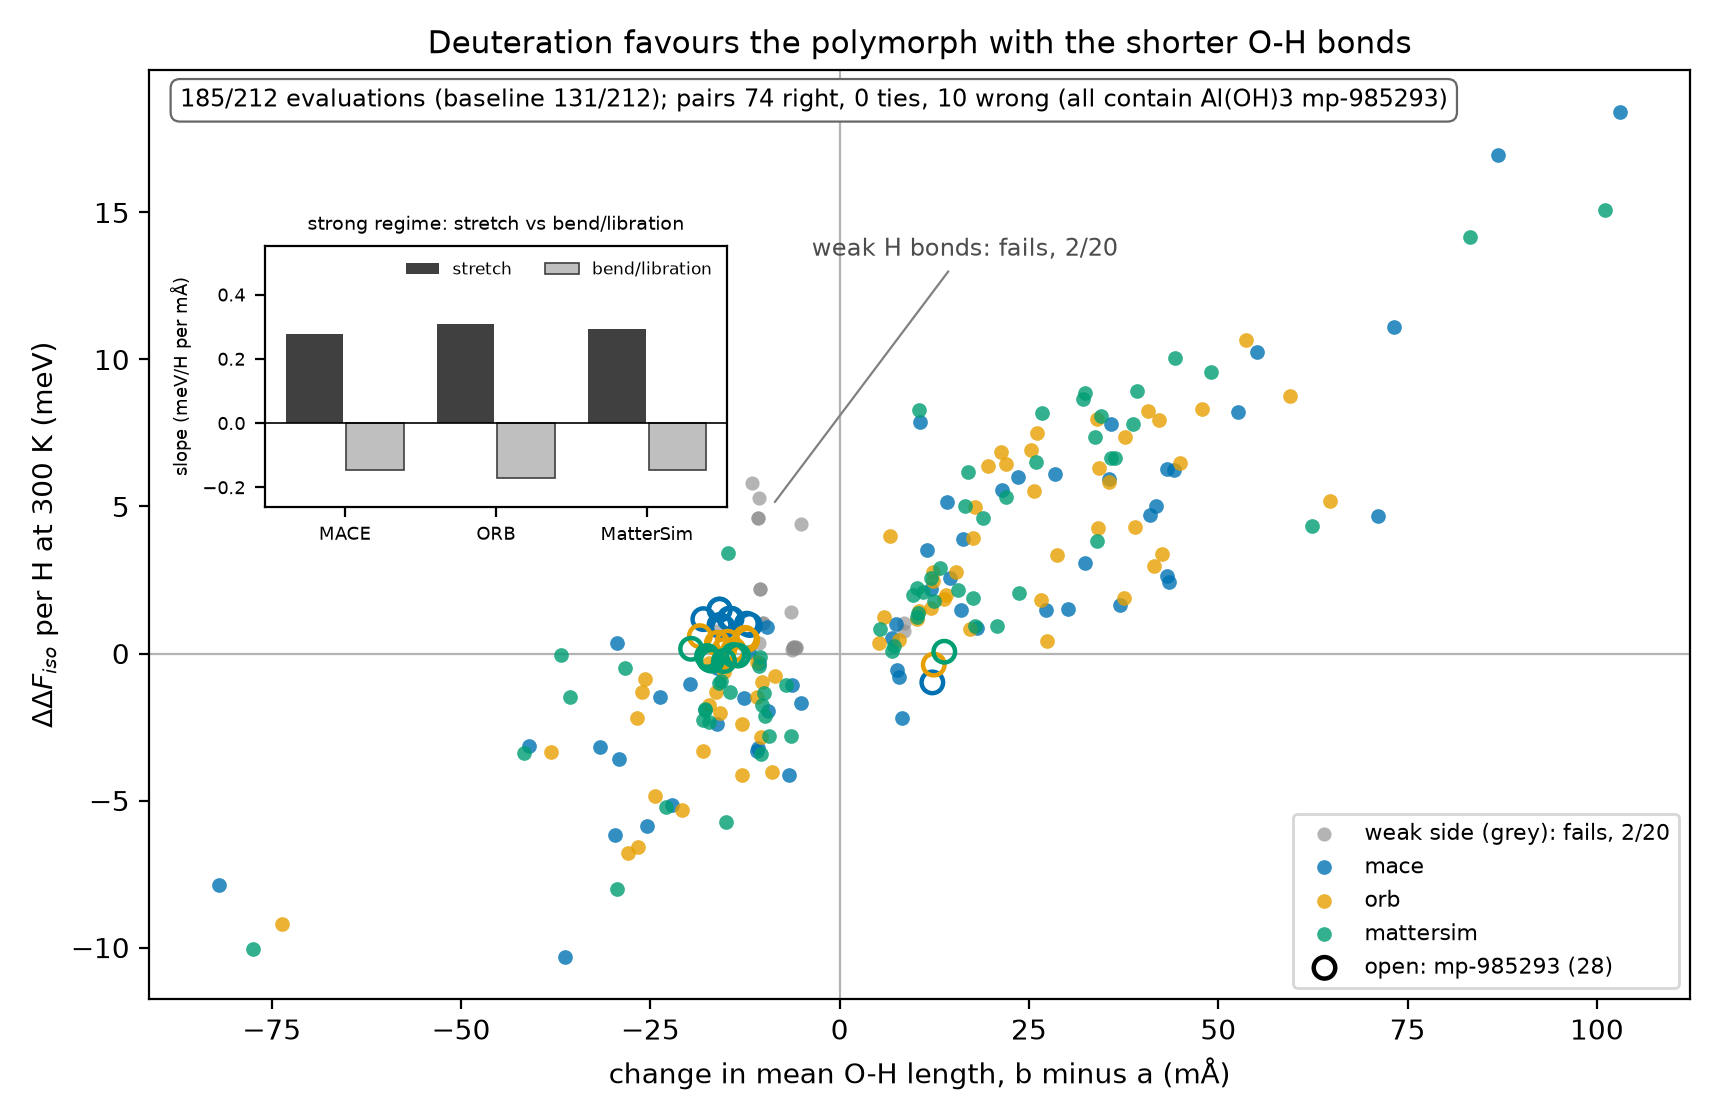
\includegraphics[width=\columnwidth]{figures/fig_headline.png}
\caption{The short-bond rule. Each point is one O-H pair computed with one model, with $|\Delta$ mean O-H$|\geq 5$~m\AA. The horizontal axis is the change in mean model O-H length from polymorph $a$ to $b$; the vertical axis is $\ddF$ per H at 300~K. Points in the upper right and lower left quadrants follow the rule. Regime by the larger mean model O-H of the pair: coloured points have $r_{\max}\geq0.99$~\AA{}, grey points (weak hydrogen bonds) are below it. The 0.99~\AA{} boundary was chosen after inspecting the data; nested re-choice picks 1.00~\AA{} in 30 of 31 folds. Open markers are the 28 evaluations involving Al(OH)$_3$ mp-985293, kept in every count. Inset: fitted slopes of the stretch term and of the bend and libration term in the strong O-H regime. Evaluations share structures and models.}
\label{fig:headline}
\end{figure}

\subsection{Slope of the isotope term against bond length}
\label{sec:slope}

Across the 220 pairs, $\ddF$ per H at 300~K is close to linear in the change of mean X-H length (Fig.~\ref{fig:allrows}a, Table~\ref{tab:models}). The fitted slopes over all clean covalent rows are 0.112 (MACE), 0.117 (ORB) and 0.128 (MatterSim) meV per H per m\AA, with Pearson $r$ of 0.76, 0.83 and 0.84. A positive slope means that the polymorph with the longer X-H bonds, which in hydrogen-bonded solids is the one with the stronger hydrogen bonds, is destabilised by deuteration. A difference of 10~m\AA{} in mean O-H length shifts the H/D free-energy balance by about 1.1 to 1.3~meV per H; for scale, the median difference between Materials Project O-H polymorphs is 4.1~m\AA{} in database geometries. These slopes are associations across polymorph pairs, not derivatives obtained by stretching one structure. A longer covalent O-H bond corresponds here to a stronger hydrogen bond and a shorter donor-acceptor O$\cdots$O distance; the two lengths should not be conflated.

The mode-resolved integral attributes the slope to two opposing terms (Fig.~\ref{fig:allrows}b). Over all rows the stretch term has a slope of $+0.245$ (MACE), $+0.259$ (ORB) and $+0.252$ (MatterSim) meV per H per m\AA{} and the bend and libration term $-0.133$, $-0.142$ and $-0.124$, so 49 to 55\% of the stretch slope is cancelled. In the O-H strong regime defined below the total slopes are 0.132, 0.136 and 0.147, the stretch slopes 0.277, 0.308 and 0.293, and the bend and libration slopes $-0.145$, $-0.171$ and $-0.146$, a compensation of 0.52, 0.56 and 0.50 (MACE, ORB, MatterSim). The two populations differ and are quoted separately. SevenNet, used for sign votes only, has 23 clean covalent rows and an all-row slope of 0.10; it is drawn in Fig.~\ref{fig:allrows} for comparison and not used in any claim.

\begin{figure*}[t]
\centering
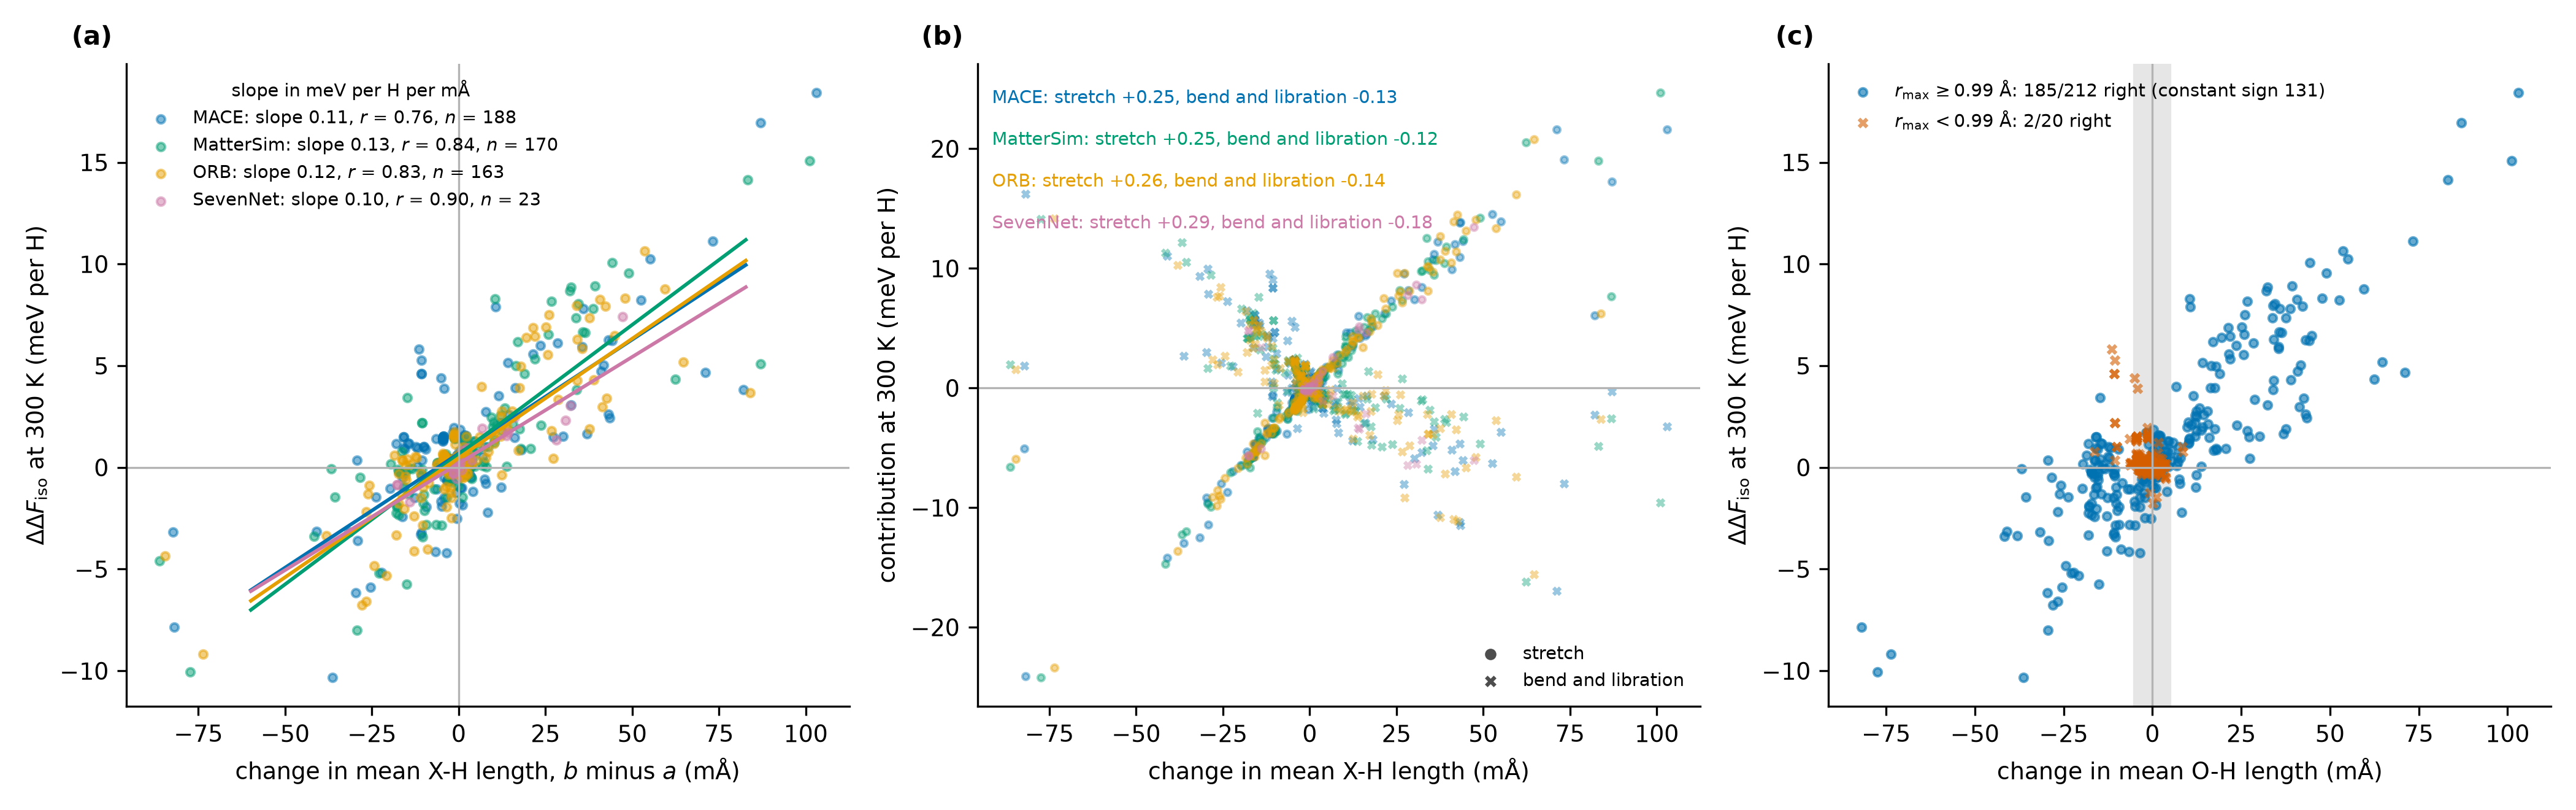
\includegraphics[width=\textwidth]{figures/fig4_xh_rule.png}
\caption{All clean covalent rows of the screen at 300~K. (a) $\ddF$ per H against the change in mean X-H length with per-model least-squares lines; legends give slope, $r$ and the number of rows (SevenNet drawn for comparison only). (b) Mode-resolved stretch contribution (circles) and bend and libration contribution (crosses) against the same axis, with per-model slopes. (c) O-H pairs without a cut on $|\ddF|$: blue, at least one polymorph with mean model O-H $\geq0.99$~\AA{} (185 of 212 right, baseline 131); orange, both below (2 of 20 right). The grey band marks $|\Delta|<5$~m\AA, excluded from the sign test.}
\label{fig:allrows}
\end{figure*}

\begin{table*}[t]
\caption{Per-model slopes and counts. Slopes in meV per H per m\AA{} at 300~K. All-row values are fits over all clean covalent rows of the screen; strong-regime values are O-H rows with $r_{\max}\geq0.99$~\AA. Sign counts use O-H pairs with $r_{\max}\geq0.99$~\AA{} and $|\Delta|\geq5$~m\AA{}, no cut on $|\ddF|$. Temperatures other than 300~K are post-freeze rescorings at fixed geometry (Sec.~\ref{sec:temperature}).}
\label{tab:models}
\begin{ruledtabular}
\begin{tabular}{lcccc}
 & MACE & ORB & MatterSim & Pooled \\
\hline
Clean covalent rows & 188 & 163 & 170 & 521 \\
All-row slope & 0.112 & 0.117 & 0.128 & \\
Pearson $r$ (all rows) & 0.76 & 0.83 & 0.84 & \\
All-row stretch / bend and libration & $+0.245$ / $-0.133$ & $+0.259$ / $-0.142$ & $+0.252$ / $-0.124$ & \\
All-row compensation & 54\% & 55\% & 49\% & \\
Strong-regime rows in fit & 97 & 97 & 99 & \\
Strong-regime total slope & 0.132 & 0.136 & 0.147 & \\
Strong-regime stretch / bend and libration & 0.277 / $-0.145$ & 0.308 / $-0.171$ & 0.293 / $-0.146$ & \\
Strong-regime compensation & 0.52 & 0.56 & 0.50 & \\
Sign rule right, 300~K & 52/68 & 64/73 & 69/71 & 185/212 \\
Constant-sign baseline, 300~K & & & & 131/212 \\
Sign rule right, 0~K & 44/68 & 54/73 & 55/71 & 153/212 \\
Sign rule right, 600~K & 67/68 & 73/73 & 70/71 & 210/212 \\
Stretch slope ratio $f$ vs Libowitzky, 2.50 to 2.80~\AA & 0.91 & 0.92 & 0.92 & \\
Isotope ZPE difference MAE vs DFT (meV per H) & 1.5 & 0.7 & 1.3 & \\
\end{tabular}
\end{ruledtabular}
\end{table*}

\subsection{The sign rule}
\label{sec:sign}

The slope suggests a sign rule: deuteration favours the polymorph with the shorter O-H bonds. The frozen statement of the result is as follows. When at least one polymorph has a mean model O-H length of 0.99~\AA{} or more (a model-derived boundary for moderate to strong hydrogen bonds, chosen after inspecting the data), deuteration favours the polymorph with the shorter O-H bonds in 185 of 212 O-H model evaluations with $|\Delta$ mean O-H$|\geq5$~m\AA{} (84 pairs, 28 formulas), against 131 of 212 for a constant-sign baseline fitted on leave-one-formula-out training folds. By model majority 74 pairs are right and 10 are wrong, with no ties, and all 10 wrong pairs contain one Al(OH)$_3$ structure, mp-985293 (Fig.~\ref{fig:headline}).

Per model the rule is right in 52 of 68 MACE, 64 of 73 ORB and 69 of 71 MatterSim evaluations. SevenNet gets 10 of 10 on the same population (baseline 7 of 10); as a fourth vote the count is 195 of 222 against 138, with 75 pairs right and the same 10 wrong. Without any threshold the rule holds in 187 of 232 O-H evaluations (81\%). The evaluations share structures and models, and the three potentials are separate models rather than independent validations, so the pair-majority count is the more conservative unit.

The boundary was chosen after inspecting the data. Re-choosing it inside each leave-one-formula-out training fold picks 1.00~\AA{} in 30 of 31 folds and 0.99~\AA{} only in the fold that holds out Al(OH)$_3$, and gives 183 of 210 held-out evaluations right against a baseline of 131. In that Al(OH)$_3$ fold the rule scores 8 of 28 against a baseline of 19, so a sharp, universal boundary is not established. A structure-only version that needs no phonons, using mean O$\cdots$O $\leq2.93$~\AA{} as the regime and the sign of the O$\cdots$O difference, is weaker: 187 of 241 evaluations with $|\ddF|>0.1$~meV per H (78\%) against a baseline of 61\%.

\textit{The Al(OH)$_3$ exception.} Structure mp-985293 is a 28-atom $P2_12_12_1$ polymorph of Al(OH)$_3$ listed by the Materials Project as experimental, with no imaginary modes in any of the three models. Its mean model O-H of 0.996 (MACE), 0.997 (ORB) and 0.999~\AA{} (MatterSim) sits just above the boundary, while its individual donors span 0.987 to 1.005~\AA{} and its mean O$\cdots$O contacts, 2.77 to 2.82~\AA, are shorter than those of its partners; it is also denser, 6.79 to 6.94~\AA$^3$/atom against 7.54 to 7.88 for every partner. In its 28 headline evaluations the stretch term has the predicted sign, but bend and libration cancel 95 to 132\% of it instead of about half (MACE 1.19 to 1.32, ORB 1.02 to 1.14, MatterSim 0.95 to 1.03, against a median of 0.50 in the other strong-regime rows). MACE calls 0 of 10 of its pairs right, ORB 0 of 9 and MatterSim 8 of 9, with every MatterSim value at $|\ddF|\leq0.26$~meV per H. This structure marks where bond length alone stops predicting the sign: when bend and libration outweigh the stretch, the rule fails even though the stretch term behaves as expected. We do not claim a phase identity or a mechanism for its larger compensation. A post-freeze test of whether the mean O-H$\cdots$O angle predicts the excess compensation failed its predeclared criterion and did not beat the bare rule on the three models (Table~\ref{tab:tests}).

Two numerical diagnostics are reported, not used as filters. One concerns a flag: 42 of the 212 headline evaluations carry a stored classical-limit flag, including all 28 that involve mp-985293; mp-985293 itself has no imaginary modes, so the flag on those rows comes from its partners or from flags kept across refinement passes. The flag fires when $|\ddF(2000~\mathrm{K})| > |\ddF(600~\mathrm{K})|$, which a sign change with temperature produces by construction (Sec.~\ref{sec:temperature}). The other is a pair of post hoc locators, chosen after seeing the frozen data: leaving out the 10 pairs with mp-985293 gives 177 of 184, and raising the boundary to 1.00~\AA{} gives 175 of 182. These are nearly the same intervention, because 28 of the 30 evaluations between 0.99 and 1.00~\AA{} come from mp-985293. Neither replaces the frozen 185 of 212 or the nested 183 of 210.

\subsection{Weak hydrogen bonds}
\label{sec:weak}

Below the boundary the rule fails: when both polymorphs have mean model O-H below 0.99~\AA, it is right in 2 of 20 evaluations (13 pairs, 7 formulas; grey points in Fig.~\ref{fig:headline}). The failures are not from one formula. In this regime the measured stretch frequency changes little with hydrogen-bond length (the Libowitzky curve spans only 170~cm$^{-1}$ from 2.80 to 3.10~\AA), so the stretch term is small and other terms can set the sign; which ones was not tested. The rule is therefore limited to moderate and strong hydrogen bonds. Whether the weak side shows a reversed law or only no skill is not established by 20 evaluations.

\subsection{The stretch term against measured spectra}
\label{sec:stretch}

\begin{figure}[t]
\centering
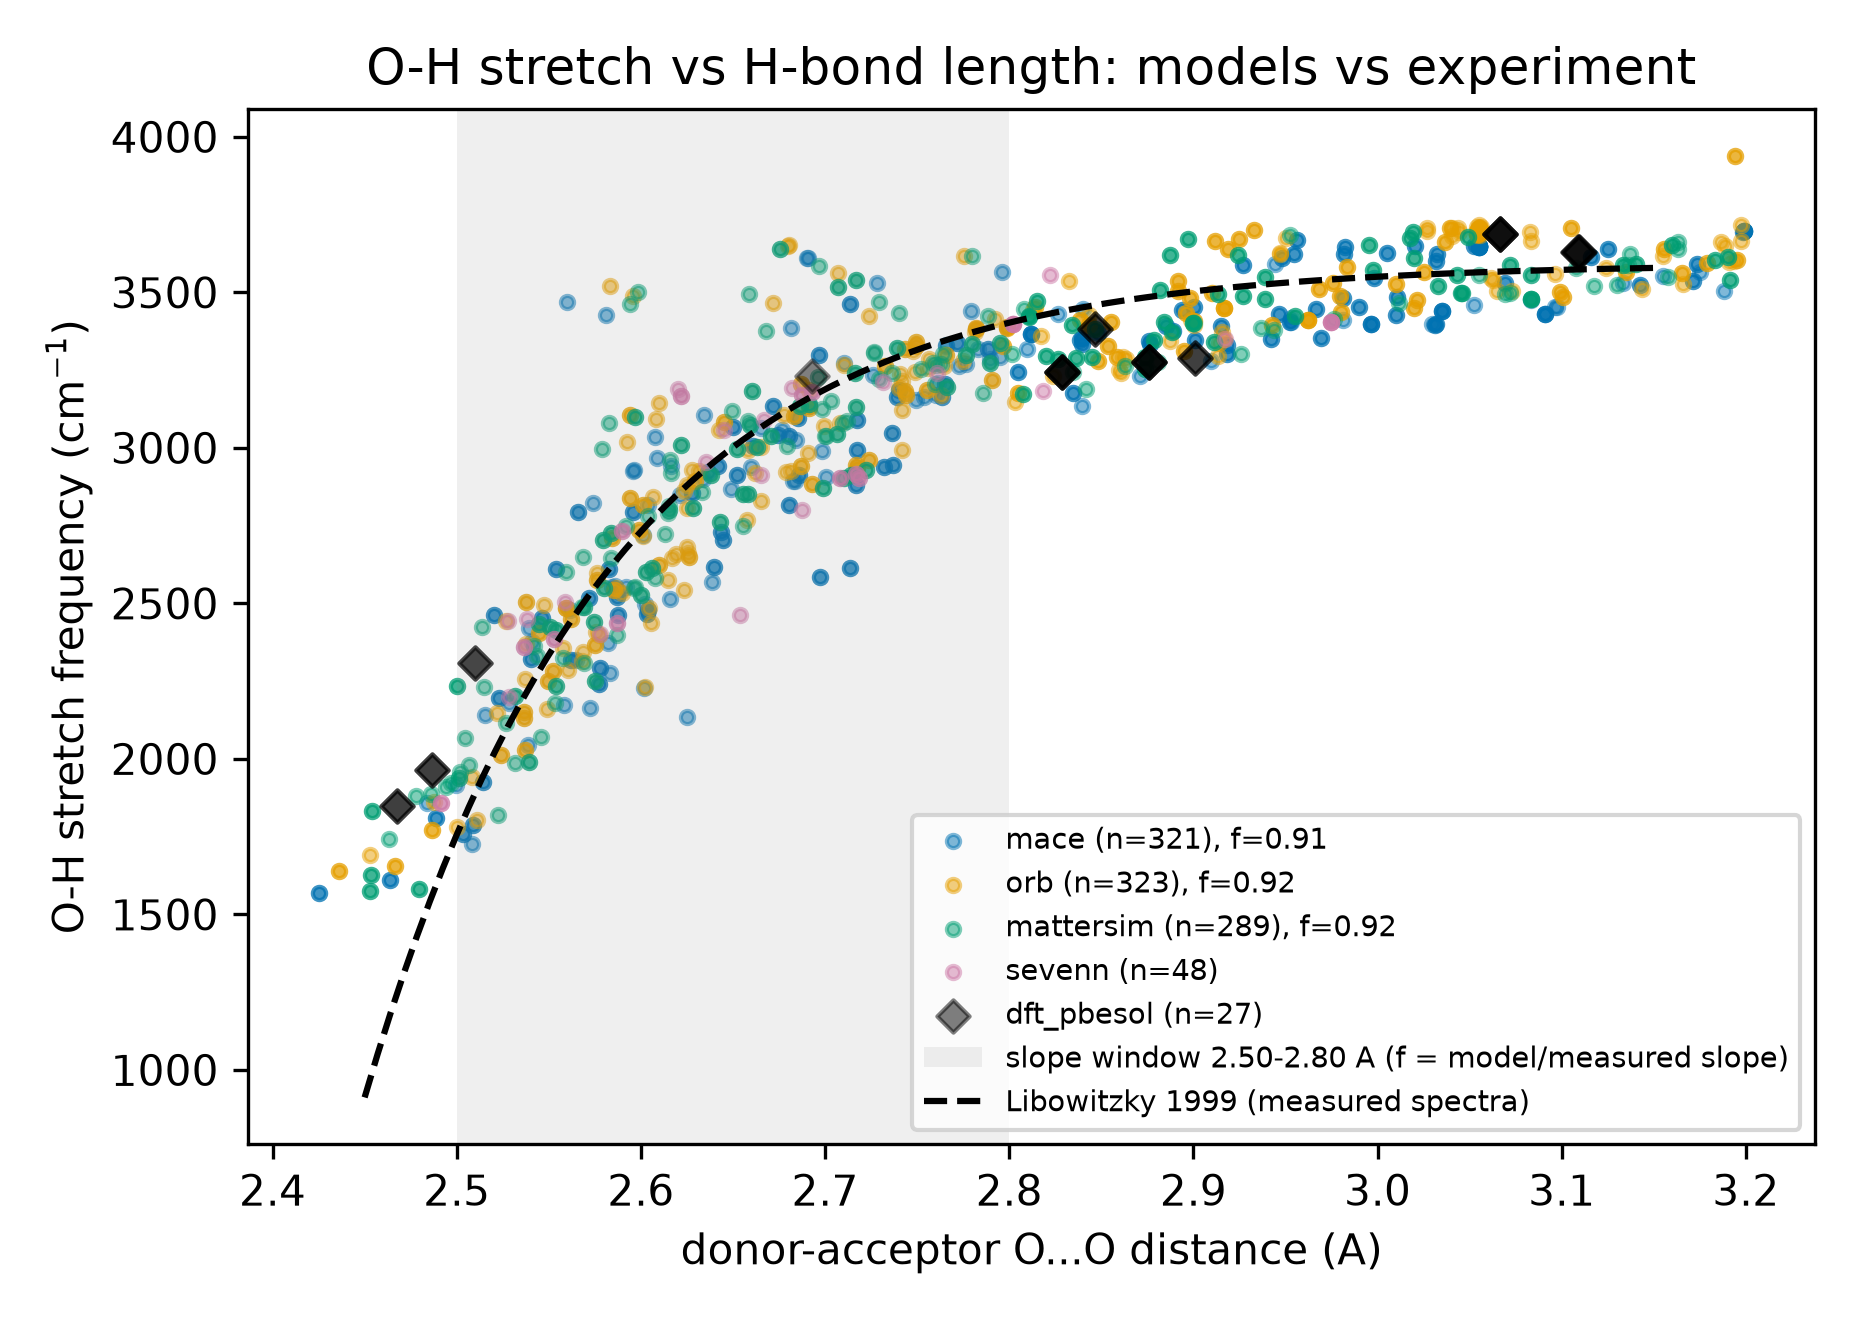
\includegraphics[width=\columnwidth]{figures/fig5_stretch_check.png}
\caption{Harmonic $\Gamma$-point O-H stretch frequencies of the model donors against donor-acceptor O$\cdots$O distance, with the empirical correlation of Libowitzky built from measured spectra~\cite{Libowitzky1999} (dashed) and PBEsol phonons of 27 donors (diamonds). The shaded window, 2.50 to 2.80~\AA, is where the slope ratio $f$ (model over measured slope) is evaluated. Harmonic model frequencies are compared with anharmonic measured fundamentals.}
\label{fig:stretch}
\end{figure}

The slope rests on how the stretch frequency changes with hydrogen-bond geometry, which can be compared with measurements. For O-H donors with model O$\cdots$O distances of 2.50 to 2.80~\AA, the harmonic $\Gamma$-point stretch frequencies follow the slope of the Libowitzky correlation~\cite{Libowitzky1999} with slope ratios of 0.91 (MACE, 52 donors in 18 structures), 0.92 (ORB, 58 in 20) and 0.92 (MatterSim, 58 in 17), with bootstrap 95\% intervals of 0.67 to 1.07, 0.82 to 1.01 and 0.81 to 1.02 (Fig.~\ref{fig:stretch}). The measured curve spans 1646~cm$^{-1}$ in this window. Because the model frequencies are harmonic and the measured ones are fundamentals, and the gap between the two grows with hydrogen-bond strength, the harmonic reference slope is flatter than the measured one; with an assumed growth of that gap by 150 to 400~cm$^{-1}$ over the window, the corrected ratios are 1.00 to 1.22. The rule would change sign only for ratios of about 1.9 to 2.3. Above 2.80~\AA{} the ratios are 0.67, 2.61 and 1.46, so ORB and MatterSim are too steep there, and the strong regime reaches O$\cdots$O of about 2.93~\AA{}, so the last 0.13~\AA{} of the regime is not covered by the check. This is a consistency check on the stretch term, not a validation of isotope free energies, and it says nothing about the bend and libration term.

\subsection{Temperature dependence}
\label{sec:temperature}

The isotope free energies stored before the freeze at 0, 300, 600 and 2000~K allow the same 212 evaluations to be rescored at other temperatures at fixed geometry. This rescoring is post hoc; the mechanism was then tested with four hypotheses committed before any new decomposition run. The sign rule is right in 153, 185 and 210 of 212 evaluations at 0, 300 and 600~K (Table~\ref{tab:models}), against leave-one-formula-out baselines of 145, 131 and 114. At 0~K the rule barely beats the baseline: it is a thermal rule. The 28 mp-985293 rows score 0, 8 and 28 of 28 at 0, 300 and 600~K. All 212 rows pass the quadrature check at 0 and 300~K and 190 at 600~K (24 of the 28 mp-985293 rows), where omitted soft modes weigh more; quadrature and direct $\ddF$ have the same sign in all 212 rows at every temperature, so the counts do not depend on the numerical route.

Of the four predeclared hypotheses, three passed and one failed. The stretch term keeps the predicted sign in all 28 mp-985293 rows at 0 and 600~K, with compensation above 1 at 0~K and below 1 at 600~K (28 of 28, passed); these rows therefore cross over in temperature rather than through a change of the stretch sign. The crossover lies between 431 and 506~K for MACE, 317 and 406~K for ORB and mostly below 300~K for MatterSim (descriptive, not predeclared). The Teller-Redlich product rule holds at every $q$ to $2.6\times10^{-11}$ per H in these structures (passed), so the mass scaling is intact. At 2000~K the sign of $\ddF$ equals the sign predicted by the change in the trace of the on-site H force constants in 211 of 212 rows (bar 202, passed); this test initially scored 124 of 212 because the scoring script read the pair orientation from the wrong file, and it was rescored after that fix with the hypothesis, threshold and rows unchanged. With the stretch near 5000~K, $\hbar\omega/k_{\mathrm{B}}T$ is still about 2.5 at 2000~K, so this is a sign test, not evidence that every mode is classical. The polymorph with the shorter mean O-H has the larger H force-constant trace in all 212 rows. The hypothesis that failed was the proposed reason for the temperature trend: compensation falls with temperature in 198 of 212 rows, but by about 39\% at the median between 0 and 600~K (median $C$ 0.665, 0.582 and 0.406 at 0, 300 and 600~K), and the predeclared drop of more than 40\% in at least 80\% of rows was met in only 98 of 212. The temperatures above about 500~K describe the harmonic isotope term at fixed geometry, not phase stability; gibbsite and many hydrates decompose below 600~K.

\subsection{Analytic estimate of the slope}
\label{sec:analytic}

The following estimate was derived after submission of the screen and changes no frozen number. For one harmonic mode, $F = k_{\mathrm{B}}T\ln[2\sinh(\hbar\omega/2k_{\mathrm{B}}T)]$, and the isotope ratio of an O-H stretch is $\rho = \omega_{\mathrm{H}}/\omega_{\mathrm{D}} = \sqrt{\mu_{\mathrm{D}}/\mu_{\mathrm{H}}}$ with the reduced masses of $^{16}$O with H and D, $\rho = 1.373607$ and $1/\rho = 0.728010$. Using $1/\sqrt{2}$ instead overstates every shift by 7\%. Let $s = -d\nu_{\mathrm{str}}/dr_{\mathrm{OH}}$ be the softening of the stretch wavenumber as the O-H bond lengthens. Linearising $\ddF$ in the bond-length difference gives the stretch slope
\begin{equation}
S_{\mathrm{str}} = \frac{hc}{2}\,s\left[\coth\frac{x}{2} - \frac{1}{\rho}\coth\frac{x}{2\rho}\right] \simeq \frac{hc}{2}\left(1 - \frac{1}{\rho}\right)s ,
\label{eq:Sstr}
\end{equation}
with $x = hc\nu_{\mathrm{H}}/k_{\mathrm{B}}T$. For stretch wavenumbers of 3000 to 3600~cm$^{-1}$ the bracket equals its zero-temperature value to better than $5\times10^{-5}$ at 300~K, so $S_{\mathrm{str}} = 0.016861\,s$~meV per H per m\AA{} with $s$ in cm$^{-1}$ per m\AA. The sign follows directly: a longer O-H bond softens the stretch, which makes $F_{\mathrm{D}} - F_{\mathrm{H}}$ less negative, so from the stretch alone deuteration favours the polymorph with the shorter O-H bond.

The one empirical input is $s$. From the screen's own phonons (donors with stretch weight above 0.5 and mean O-H of 0.96 to 1.05~\AA), the model stretch frequencies fall by 19.0 (MACE), 19.3 (ORB) and 19.5 (MatterSim) cm$^{-1}$ per m\AA, with $r = -0.99$ to $-1.00$; narrower windows give 17 to 21. An experimental value of $d\nu/dr_{\mathrm{OH}}$ was not checked against a primary source and is not used. With $s = 19$ to 19.5, Eq.~\eqref{eq:Sstr} gives $S_{\mathrm{str}} = 0.32$ to 0.33~meV per H per m\AA, against the mode-resolved stretch slopes of 0.25 to 0.31 fitted in Sec.~\ref{sec:slope}. The one-mode estimate is 5 to 30\% high. Two likely reasons, not tested here, are that the regressor in the screen is the mean O-H length of all H in the cell while $s$ is fitted per donor, and that the stretch is not a pure mode, so part of its shift sits in mixed modes counted as bend.

Bends and librations harden as the hydrogen bond strengthens. With $s_b = +d\nu_b/dr_{\mathrm{OH}}$ for each of $n_b = 2$ bending modes per H, the bend term is $S_{\mathrm{bend}} = -n_b s_b (hc/2)[\coth(x_b/2) - \rho_b^{-1}\coth(x_b/2\rho_b)]$, and at 0~K with $\rho_b \approx \rho$ the compensation is $f = n_b s_b/s$. The observed compensation of about 0.5 therefore requires $s_b \approx s/4$, roughly 5~cm$^{-1}$ per m\AA{} per bend for $s = 19$. This value is inferred from the compensation, not measured. Temperature acts on the two terms differently. Relative to 0~K the stretch weight is 1.000 at 300~K and 0.988 at 600~K, while a 1200~cm$^{-1}$ bend falls to 0.941 and 0.687 and a 900~cm$^{-1}$ libration to 0.858 and 0.556. With $s = 18$, $s_b = 4.5$ and $\nu_b = 1400$~cm$^{-1}$, $f$ falls from 0.50 at 0~K to 0.48 at 300~K and 0.38 at 600~K and the net slope rises from 0.15 to 0.16 and 0.19. At high temperature the sign is set by one monotone quantity, the H force-constant trace, while at 0~K the bend and libration cancel half of the stretch and small errors can flip signs. This agrees in direction with the rescoring of Sec.~\ref{sec:temperature}. The size of the jump from 0 to 300~K is larger than bend weights alone give and would need librations and lattice modes below about 900~cm$^{-1}$ and rows near zero; that part is a plausibility argument, not a derivation of the counts. The assumptions are harmonic modes, an isolated O-H stretch (anharmonicity, which lowers the measured O-H/O-D ratio to about 1.33 to 1.36, is outside the estimate), linear dependence of frequencies on O-H length over the range used, and bends treated as two modes of one frequency.

The direction of the rule and the size of the stretch slope thus follow from harmonic physics and one empirical relation. What the screen adds is the outcome of the stretch against bend and libration competition at room temperature across real polymorph pairs, its net slope, the conditions under which it fails and the prediction below.

\subsection{Prediction for diaspore and \texorpdfstring{$\delta$}{delta}-AlOOH}
\label{sec:alooh}

Diaspore ($\alpha$-AlOOH, $Pnma$, mp-625152) transforms at high pressure to $\delta$-AlOOH ($P2_1nm$, mp-23807), which has the stronger hydrogen bond: its O-H is longer by 24 to 32~m\AA{} and its O$\cdots$O shorter by 60 to 90~m\AA{} at 0~GPa in the models. The rule therefore predicts that deuteration destabilises $\delta$-AlOOH. At 0~GPa geometry, harmonic $\ddF(\delta - \mathrm{diaspore})$ at 300~K is $+0.52$, $+0.77$ and $+0.83$~meV/atom (MatterSim, MACE, ORB), with $\Delta V = -0.30$ to $-0.32$~\AA$^3$/atom, which gives $+0.3$ to $+0.4$~GPa. Quasi-harmonic Gibbs energies at 10, 15 and 20~GPa, with one linear fit for both isotopes, place the 300~K transition of AlOOD 1.33~GPa (MACE) and 1.13~GPa (ORB) above that of AlOOH, whose transition the models place at 8.76 and 13.00~GPa; the MACE AlOOH root is extrapolated below the 10~GPa grid point. The two models place the boundary 4.2~GPa apart but agree on the shift. A temperature-resolved rebuild with $\Gamma$-free meshes gives $+1.33$, $+1.13$ and $+0.99$~GPa at 300~K (MACE, ORB, MatterSim) and $+0.94$, $+0.81$ and $+0.73$~GPa at 1000~K, a shift that shrinks with temperature but keeps its sign.

This is an exploratory sign prediction outside the harmonic domain. $\delta$-AlOOH undergoes the isotope-dependent proton disorder of Ref.~\cite{SanoFurukawa2018} in the same pressure window, which harmonic physics omits, and the measured 4.4~GPa shift of that neighbouring transition shows that anharmonic isotope effects in this system are large. The experimental boundary is crossed at high temperature, and the potentials overbind hydrogen bonds (Sec.~\ref{sec:tests}). The same calculation for goethite to $\varepsilon$-FeOOH gives $+0.2$ to $+0.5$~GPa, with a $q$-mesh sensitivity as large as the signal, so only its sign is stated. A logged search found no measurement or calculation of the isotope shift of the diaspore to $\delta$-AlOOH boundary. Related measured shifts point the same way: the $\delta$-AlOOH disorder transition moves up with deuteration~\cite{SanoFurukawa2018}, and $\varepsilon$-FeOOD remains asymmetric above the pressure at which $\varepsilon$-FeOOH symmetrises~\cite{Ikeda2025}; both are proton-disorder or symmetrization transitions, not the diaspore boundary.

%=====================================================================
\section{Tests against experiment}
\label{sec:tests}

\begin{table*}[t]
\caption{Every prediction-first, blind or prospective test, with the commit that fixed the prediction before its data or result. Pre-freeze tests were scored before the headline was frozen, post-freeze tests after. ``Model'' tests compare with model or code checks, not with measurements.}
\label{tab:tests}
\begin{ruledtabular}
\begin{tabular}{p{0.07\textwidth}p{0.25\textwidth}p{0.08\textwidth}p{0.17\textwidth}p{0.36\textwidth}}
Test & What was predicted & Commit & Outcome & Notes \\
\hline
P01/F02 & Volume isotope effects of known H compounds & 0fffc54 & Mixed & $\alpha$-AlH$_3$ right sign, 1.3 to 1.5 times too large; GaOOH and $\beta$-CrOOH wrong sign against references of limited quality. Does not test the rule. \\
P02/F04 & Stretch and bend shifts, goethite to $\varepsilon$-FeOOH and diaspore to $\delta$-AlOOH & da560cf & Sign level, one pair & Goethite to $\varepsilon$-FeOOH: stretch falls, bend rises, as predicted; diaspore pair inconclusive. \\
P03/F04 & Stretch and bend shifts, manganite to groutite & c990f11 & Inconclusive & \\
P04/F05 & Harmonic mineral D/H fractionation, 118 structures & f3ac0ac & Ordering only & Signs 6 of 6 and order brucite $>$ goethite $>$ manganite right; magnitudes 5 to 10 times too large; scoring rule committed with its result (90ad4cd). \\
P05/F07 & H$_2$O to D$_2$O shift of three ice boundaries & bec68d7 & Failed & Ih-II and Ih-III wrong sign in 3 of 3 models; II-III right sign; secondary data. \\
P06/F08 & Rule refined with the O-H$\cdots$O angle & cdb32da & Failed & No gain over the bare rule; all 10 wrong pairs stay wrong. \\
P08/F10 & Structure-only atlas, 1796 pairs & d991991 & Nothing scorable & 0 of 26 literature rows usable. \\
P09/F09 & Temperature hypotheses H1 to H4 & d03f8d2 & H1 failed, H2 to H4 passed & H4 passed after a disclosed orientation fix (initial run 124 of 212). \\
P10/F11 & Prospective test on pairs never computed & eb61ccf & Failed & 16 of 111 right; 87 rows lost to predeclared numerical rules; on 24 clean rows 16 right against 19 for a constant sign. \\
P11/F12 & Boehmite against diaspore D/H fractionation & 184fbee & Inconclusive & Sign agrees at 380~$^\circ$C in 3 of 3 models; no stated uncertainty, diaspore 25\% exchanged. \\
F06 & Reimplementation without the original code & n/a & Code agrees & 9 of 9 rows to $10^{-9}$~meV/atom; tests code, not physics. \\
\end{tabular}
\end{ruledtabular}
\end{table*}

No polymorph isotope free energy has been measured, so none of the tests below scores the rule directly. Each tests an ingredient or a consequence, and Table~\ref{tab:tests} lists all of them with their outcomes.

\textit{Volume isotope effects (F02, mixed).} Quasi-harmonic volume isotope effects were predicted for known H compounds before the measured cell volumes were read. $\alpha$-AlH$_3$ has the measured sign~\cite{Turley1969} with a magnitude 1.3 to 1.5 times too large; GaOOH and $\beta$-CrOOH have the wrong sign against cross-laboratory references of limited comparability. The misses lie in the strong hydrogen-bond regime, where quasi-harmonic physics omits Ubbelohde-type proton anharmonicity. The test passed where the rule has no skill and missed where it applies, so it does not test the rule; it does show that the potentials overweight the O-H stretch contribution to volume derivatives in strongly hydrogen-bonded crystals.

\textit{Differential spectroscopy (F04, sign level, one pair).} The rule's mechanism predicts that, between two polymorphs, the stretch falls and the bend rises as the hydrogen bond strengthens. For goethite to $\varepsilon$-FeOOH the measured shifts are about $-260$~cm$^{-1}$ for the stretch, the midpoint of a broad band, so anywhere from $-511$ to $-11$~cm$^{-1}$, against $-273$ predicted, and $+290$ against $+195$~cm$^{-1}$ for the highest O-H bend~\cite{Thompson2020}. The stretch comparator is the midpoint of the broad 2600 to 3100~cm$^{-1}$ band reported for $\varepsilon$-FeOOH, not a measured peak. The goethite bands are attributed to Liu et al.~\cite{Liu2013}, whose full text was not read. Mashino et al.~\cite{Mashino2026} read the same spectrum as two maxima near 2800 to 2900 and 3300 to 3400~cm$^{-1}$; if the upper component were the main band, the stretch sign would reverse. The diaspore to $\delta$-AlOOH pair and the manganite to groutite pair were inconclusive. This is consistent with the sign of the compensating bend shift at the zone centre, not a measurement of its size; the measured bend to stretch shift ratio, about 1.1, exceeds the model median of 0.7.

\textit{Mineral D/H fractionation (F05, ordering only).} The same isotope free energies give reduced partition function ratios, so differences between measured mineral-water fractionation factors test them without a model of water. Predictions for 118 structures were committed before the data were read. The measured factors are attributed in our data file to Xu and Zheng for brucite~\cite{Xu1999}, to Yapp for goethite~\cite{Yapp1987} and to Hariya and Tsutsumi for manganite~\cite{Hariya1981}, each reached through secondary sources. The sign of every scored difference (6 of 6, in 2 scored pairs) and the order brucite $>$ goethite $>$ manganite in D affinity are right in all three models, and the mineral with the longer O-H bonds takes up less deuterium, as the rule implies. The magnitudes are not: for brucite minus goethite the models give 190 to 300 per mil against a measured 22 to 46 per mil, 5 to 10 times too large, and the predicted difference falls with temperature while the measured one rises. The preset verdict is ordering only. The three-mineral order is assembled from two temperature windows, because no temperature has all three minerals admissible, and the factor of 5 to 10 applies to brucite minus goethite; the two pairs with manganite give ratios of 1.6 and 0.7, one of them unscored. Brucite (mean O-H 0.971~\AA) lies outside the rule's regime, and the measurements were taken from secondary sources that were not checked against primary papers. The scoring rule of this test was committed together with its result, not before it.

\textit{Ice phase boundaries (F07, failed).} The H$_2$O to D$_2$O shifts of three ice boundaries were predicted before any measured D$_2$O boundary was read. For Ih-II the models give $-12$ to $-140$~MPa at 230 to 250~K, against a measured triple-point shift of $+12$ to $+15$~MPa; Ih-III is also wrong in sign in all three models, while II-III is right in sign and within a factor of 2 to 3 in size. The measured values come from a secondary compilation and from Bridgman's D$_2$O work via a reference equation of state~\cite{Bridgman1935,Herrig2018}. Both failures involve ice Ih, which is modelled through the ordered ice XI proxy, 7 to 9\% too dense in all three models. Overbound hydrogen bonds, which exaggerate the stretch term, and the omission of proton disorder are both consistent with the failure; this test cannot separate them.

\textit{Prospective test (F11, failed its bar).} After the freeze we committed signs for 111 primary evaluations of pairs never computed before (42 pairs, 20 formulas, both phases experimental), after relaxation and before any phonon run. The predeclared bar was at least 75\% right, at least 15 points above the constant-sign baseline and a pair majority right in at least 80\% of pairs. The rule got 16 of 111 right, with a baseline of 5. 87 rows were lost to the predeclared numerical rules (69 failed or dynamically unstable, 18 not clean), dominated by KH$_2$PO$_4$-type and ice polymorphs with imaginary modes, which capped the attainable accuracy at 21.6\%. The surviving rows do not rescue the rule: on the 24 clean rows it was right in 16, the precommitted constant sign in 5, and a constant guess of the opposite sign, chosen after the fact, in 19. The failure therefore combines numerical attrition with insufficient skill on the rows that survived, and transfer of the rule to new pairs is not shown. On the same clean rows, descriptively and after part of the data had been seen, the fitted total slope was 0.181 and the compensation 0.44, of the same order as in the screen. The predeclared secondary test, at 600~K without a threshold, also missed its 90\% bar (21 of 120); the 21 rows it scored right are all of its clean rows.

\textit{Boehmite against diaspore (F12, inconclusive).} Among the headline pairs only boehmite against diaspore has a measured route. The models predict that D prefers boehmite, the shorter O-H phase, by $+75.6$, $+37.3$ and $+67.9$ per mil at 300~K. Measured mineral-water fractionation~\cite{Graham1980}, read from a compilation~\cite{Chacko2001}, gives a boehmite minus diaspore difference of $+28.8$ per mil at 380~$^\circ$C, the predicted sign in all three models, but the source states no uncertainty and the diaspore value comes from 25\% exchange, so the predeclared rule scores the case inconclusive.

\textit{Reimplementation (F06).} A second model, without access to our code, rewrote the double difference and its stretch and perpendicular split from the cached force constants with its own mesh and quadrature. Of the 20 rows it computed, 9 have a reference row in our results; on these it reproduces $\ddF$ to $10^{-9}$~meV/atom with 9 of 9 signs. The other 11 belong to pairs excluded as not clean and are not validated by this check. Both codes read the same force constants, so this checks implementation and bookkeeping, not the potentials or the harmonic model.

%=====================================================================
\section{Discussion}
\label{sec:discussion}

\textit{Known physics and the new part.} The competition between stretch and bend zero-point energies in hydrogen bonds is established~\cite{McKenzie2014,McKenzie2015,Li2011}, and the high-temperature direction, in which deuterium prefers the phase with the larger H force-constant trace, is the textbook Bigeleisen-Mayer and Wigner-Kirkwood argument~\cite{Bigeleisen1947}. Hydrogen-bond control of mineral D/H fractionation is known qualitatively~\cite{Suzuoki1976,Meheut2010}, and single systems show isotopomeric polymorphism~\cite{Zhou2004,Zhou2006,Ip2012,Falk2018,Shi2018,Ford2011,Merz2015}. Section~\ref{sec:analytic} shows that the direction and the stretch slope follow from harmonic physics plus one empirical relation. What this work adds, in our reading of the literature found by a logged search, is the polymorph-stability version of the competition across many compounds: a net slope of 0.11 to 0.13~meV per H per m\AA, a sign rule with counts against a baseline, a failure boundary at weak hydrogen bonds, one structure in which bend and libration outweigh the stretch at room temperature, and a pressure prediction. The rule is best read as a physically expected effect, quantified and bounded for polymorph stability, not as an unexplained correlation. The Al(OH)$_3$ exception is informative for the same reason: its stretch term behaves as expected while the total changes sign, so a bond-length rule cannot stand for the whole vibrational free energy, and the temperature rescoring shows that one pair can change its isotope preference at fixed geometry. A shorter O-H bond goes with a weaker hydrogen bond, so in chemical terms the rule says that deuteration favours the polymorph whose hydrogen bonds are weaker, the direction seen in the pentachlorophenol and 4-methylpyridine system~\cite{Zhou2004,Ip2012}.

\textit{Limitations.} (1) The free energies are harmonic or quasi-harmonic. Anharmonicity of the O-H stretch, tunnelling and proton disorder are omitted; the tests that failed or were inconclusive (F05 magnitudes, F07, the $\delta$-AlOOH disorder window) point to exactly these effects in strongly hydrogen-bonded systems. (2) The three potentials share PBE-level training data and overbind hydrogen bonds (ice XI 7 to 9\% too dense), so a shared bias in O-H lengths would move both axes of Fig.~\ref{fig:headline} together; the stretch check bounds the slope only from 2.50 to 2.80~\AA. (3) The 0.99~\AA{} boundary was chosen after inspecting the data; nested re-choice shows that the selection effect on the count is small, but the choice of regime variable and cuts is not cross-validated, and the boundary depends on whether the Al(OH)$_3$ failure is in the training fold. (4) Evaluations share structures and models and are not independent, and the model spread is a range, not a confidence interval, so it cannot expose a bias common to all three models; the pair-majority count (74 right, 10 wrong) is the conservative unit, and the prospective test on new pairs failed its bar, through numerical losses and on the clean rows. (5) The clean criterion is narrower than physical stability: imaginary-mode treatment, incomplete relaxation and soft-mode sensitivity remain open, and the prospective test shows that they matter. (6) No polymorph isotope free energy has been measured, and no DFT double difference was computed.

\textit{The direct experiment.} D/H partitioning between two coexisting polymorphs constrains $\ddG$ directly. For polymorphs $a$ and $b$ of the same composition with $n_{\mathrm{H}}$ hydrogens per formula unit and equilibrium fractionation factor $\alpha_{a\text{-}b}$,
\begin{equation}
\ddG = n_{\mathrm{H}} k_{\mathrm{B}} T \ln\alpha_{a\text{-}b} + R ,
\label{eq:bridge}
\end{equation}
where $\alpha_{a\text{-}b}$ is the trace (dilute D) fractionation factor and $R$ accounts for the difference between trace and full substitution; with a full-substitution factor the relation is exact with $R = 0$. To second order $R \approx (n_{\mathrm{H}}k_{\mathrm{B}}T/2)[\mathrm{Var}_b(l) - \mathrm{Var}_a(l)] + N_b - N_a$, with $l_i = \ln\beta_i$ per H site and $N_p$ the non-additivity of full substitution. $R$ vanishes when the H sites are equivalent and independent with composition-independent substitution free energies and ideal mixing; harmonicity alone does not establish this, because the rule of the geometric mean needs its own assumptions~\cite{Albery1969}. Both model phases of diaspore and $\delta$-AlOOH have one inequivalent H site, so the variance term vanishes, but the non-additivity term has not been bounded, and a trace measurement constrains the predicted full-substitution difference only once it is. Equation~\eqref{eq:bridge} is the solid-state analogue of the Bigeleisen relation between vapour-pressure isotope effects and fractionation~\cite{Bigeleisen1947}. The boundary shift then follows as $\Delta P_{\mathrm{iso}} \approx -\ddG/\Delta V$ to linear order. For diaspore and $\delta$-AlOOH, a shift of $+1.2$~GPa at 300~K corresponds to $1000\ln\alpha(\mathrm{diaspore} - \delta) = +359$ per mil; given the 5 to 10 times overestimate of harmonic fractionation magnitudes in F05, the measured value may well be smaller, which is why only the sign is predicted. The second test is a matched, reversed-bracket determination of the diaspore to $\delta$-AlOOH boundary for AlOOH and AlOOD in the same press, pressure medium, calibrant and temperature path, with each boundary approached from both phase assemblages. A shift of opposite sign contradicts the prediction; a shift not resolvable from zero is a null result.

%=====================================================================
\section{Conclusion}
\label{sec:conclusion}

In harmonic calculations with three universal ML potentials over 220 polymorph pairs, the H/D free-energy difference between polymorphs follows the change in mean X-H bond length with a slope of 0.11 to 0.13~meV per H per m\AA, a stretch term about half cancelled by bend and libration. In crystals with moderate to strong hydrogen bonds, deuteration favours the polymorph with the shorter O-H bonds in 185 of 212 model evaluations against 131 for a constant-sign baseline; the rule fails for weak hydrogen bonds and in one Al(OH)$_3$ structure where bend and libration outweigh the stretch at room temperature, and it did not transfer in a prospective test whose rows were mostly lost to numerical rules. A one-mode harmonic estimate reproduces the sign and, within 5 to 30\%, the size of the stretch slope from the stretch softening alone. The rule predicts that deuteration raises the diaspore to $\delta$-AlOOH transition by about 1~GPa. D/H partitioning between coexisting polymorphs and matched AlOOH and AlOOD boundary runs would test it.

%=====================================================================
\section*{Data and code availability}

Code, data, prediction files, decision records and findings are at \url{https://github.com/canerganis/isoshift}~\cite{IsoShiftGitHub}. The version submitted to the OSI Hackathon 2026 is archived as v1.0.0 at Zenodo, doi:\href{https://doi.org/10.5281/zenodo.23578412}{10.5281/zenodo.23578412}~\cite{IsoShiftZenodo}. The headline counts are recomputed on a CPU in seconds from the frozen pair table with \texttt{python -m src.isoshift\_event.rule\_cv}. The post-freeze analyses (F09, F11, F12) were committed on 22 October 2026, before the DOI was added to the repository; the analytic estimate of Sec.~\ref{sec:analytic} (note M03 and its check script) was committed on 23 October 2026, after the archived release, and is not part of v1.0.0. Derived Materials Project data are CC BY 4.0; the licence of the redistributed JARVIS-DFT structures was not verified.

\begin{acknowledgments}
The author thanks the organisers of the OSI Hackathon 2026, Ben Blaiszik and colleagues, for the event in which this work was done; Valency Systems for access to the Valency Bond literature service; and the marimo team for the notebook framework used for the results application.
\end{acknowledgments}

\section*{AI-use statement}

AI agents did the work under the author's direction, each with a fixed role; the author set the question, approved each step and made the calls that needed a person.
(1) Conductor: Claude Opus 5.5 planned the work, ran the GPU screen with MACE, ORB, MatterSim and SevenNet, wrote the analysis and kept a ledger of every step.
(2) Literature and blind-test agents: Claude Sonnet instances queried Valency Bond, each with one task (a validation value, an ice boundary, a fractionation factor); the blind-test agents never saw the predictions.
(3) Math checks: every formula was derived twice, independently, by GPT-6 Astra and Claude Opus, and the code used it only after the two agreed.
(4) Councils: hard calls (the freeze, what to claim, what to drop) went to a council of Claude Opus, GPT-6 Astra and Gemini 4 Argon. Each member answered blind, then read and challenged the others; the chair (Claude Opus) decided by argument, not vote, and recorded the dissent.
(5) Independent check: GPT-6 Astra, through Codex and without our code, rewrote the calculation from the equations and matched $\ddF$ to $10^{-9}$~meV/atom, which checks the code, not the physics.
After submission, Claude Haiku agents ran the two prior-art search rounds, and the analytic estimate of Sec.~\ref{sec:analytic} was derived independently by GPT-6 Astra and Claude Opus and cross-checked numerically. This manuscript was drafted from the repository records by Claude Opus 5.5, which merged in parts of an independent draft by GPT-6 Astra. Agreement between agents is not treated as experimental validation. The author is responsible for the content.

\bibliography{refs}

\appendix

\section{Pipeline counts}

\begin{figure}[h]
\centering
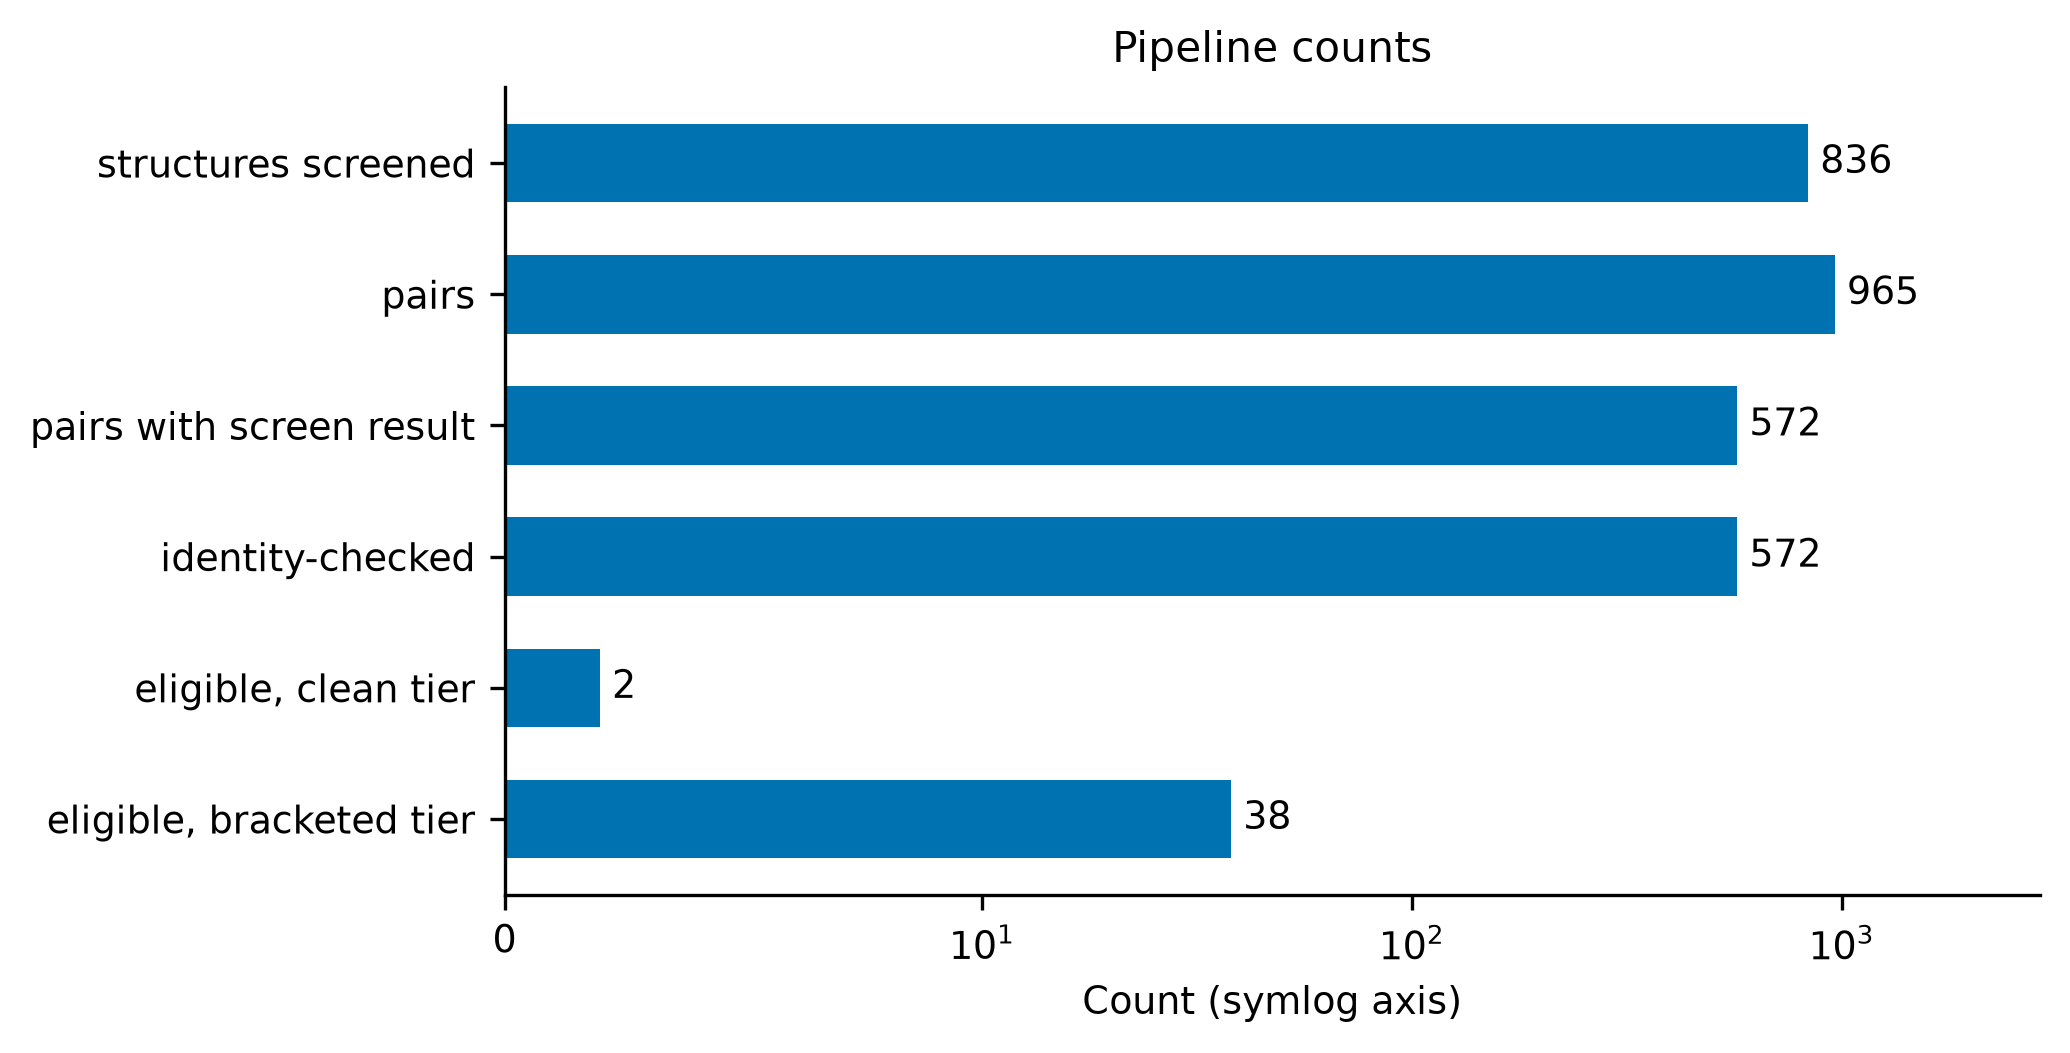
\includegraphics[width=\columnwidth]{figures/fig2_pipeline_counts.png}
\caption{Pipeline counts on a symmetric-log axis: 836 structures, 965 polymorph pairs, 572 pairs with a screen result in at least one model, all of which passed the structural identity check. The two lower bars count candidate pairs for boundary-shift cards in two quality tiers and are not used in this paper. Of the 965 pairs, 220 (63 formulas) have clean covalent X-H results and enter the slope fit, and 84 O-H pairs enter the headline sign test.}
\label{fig:pipeline}
\end{figure}

\end{document}
